\documentclass{article}
\usepackage[parfill]{parskip}
\usepackage{adjustbox}
\usepackage{listings}
\usepackage{graphicx}
\usepackage{color}
\usepackage{hyperref}
\usepackage{tikz}
\usetikzlibrary{shapes.geometric, arrows, positioning}
\tikzstyle{startstop} = [rectangle, rounded corners, minimum width=3cm, minimum height=1cm,text centered, draw=black, fill=red!30]
\tikzstyle{io} = [trapezium, trapezium left angle=70, trapezium right angle=110, minimum width=3cm, minimum height=1cm, text centered, draw=black, fill=blue!30]
\tikzstyle{process} = [rectangle, minimum width=3cm, minimum height=1cm, text centered, draw=black, fill=orange!30, text width=3cm]
\tikzstyle{decision} = [diamond, minimum width=3cm, minimum height=1cm, text centered, draw=black, fill=green!30]
\tikzstyle{arrow} = [thick,->,>=stealth]
\hypersetup{
	colorlinks,
	citecolor=black,
	filecolor=black,
	linkcolor=black,
	urlcolor=black
}
\graphicspath{ {img/} }

\lstset{basicstyle=\ttfamily,
  mathescape=true,
  escapeinside=||}

\begin{document}
\title{COMP33711 - Agile Software Engineering}
\author{Christopher Williamson}
\maketitle
\tableofcontents
\newpage
\section{Introduction}
`We are uncovering better ways of developing software by doing it and helping others to do it. Through this work we have come to value:
\begin{itemize}
	\item \textbf{Individuals and interactions} over processes and tools.
	\item \textbf{Working software} over comprehensive documentation.
	\item \textbf{Customer collaboration} over contract negotiation.
	\item \textbf{Responding to change} over following a plan.
\end{itemize}
That is, while there is value in the items on the right, we value items on the left more.'
\subsection{Key Ideas for Agile Approaches}
One of the key ideas is to avoid waste which commits people to delivering real value. Trust is also a key idea. This includes having a self-organising team, empowering developers to make key decisions and including the customer as a member of the team. Simplicity of both the process and product is important. YAGNI (You Aren't Gonna Need It) is a principle that is often followed which basically means that a programmer should not add functionality until deemed necessary.

Finally, feedback is another key idea. We should aim to `fail fast' by making sure that failure is visible quickly. Short iteration, close customer involvement in development, team retrospectives, high-coverage automated test suites and pair programming are all useful idea that aid the feedback process.

\subsection{12 Agile Principles}
To help people gain a better understanding of what agile software development is all about, the members of the agile alliance refined the philosophies captured in their manifesto into a collection of twelve principles:
\begin{enumerate}
	\item Our highest priority is to satisfy the customer through early and continuous delivery of valuable software.
	\item Welcome changing requirements, even late in development. Agile processes harness change for the customer's competitive advantage.
	\item Deliver working software frequently, from a couple of weeks to a couple of months, with a preference to the shorter time scale.
	\item Business people and developers must work together daily throughout the project.
	\item Build projects around motivated individuals. Give them the environment and support they need, and trust them to get the job done.
	\item The most efficient and effective method of conveying information to and within a development team is face-to-face conversations.
	\item Working software is the primary measure of progress.
	\item Agile processes promote sustainable development. The sponsors, developers, and users should be able to maintain a constant pace indefinitely.
	\item Continuous attention to technical excellence and good design enhances agility.
	\item Simplicity - the art of maximising the amount of work not done - is essential.
	\item The best architectures, requirements, and designs emerge from self-organising teams.
	\item At regular intervals, the team reflects on how to become more effective, then tunes and adjusts its behaviour accordingly.
\end{enumerate}

\subsection{N Agile Practices}
There is no limit on agile practices but some examples are short iterations, user stories, story points, planning games and TDD.

\subsection{M Agile Methodologies}
As above, there is no limit on agile methodologies but some examples are eXtreme Programming (XP), Scrum and Crystal.

\subsection{Waterfall VS Agile}
When using the waterfall approach, we usually have the following structure:\\\\
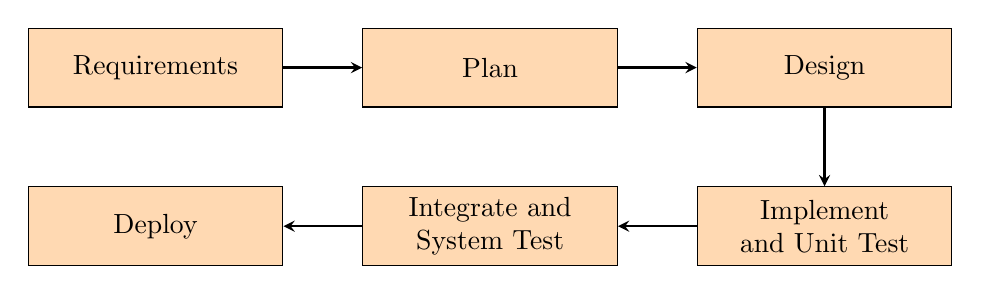
\begin{tikzpicture}[node distance=1cm]
	\node (reqs) [process] {Requirements};
	\node (plan) [process, right= of reqs] {Plan};
	\node (design) [process, right=of plan] {Design};
	\node (unittest) [process, below=of design] {Implement and Unit Test};
	\node (systemtest) [process, left=of unittest] {Integrate and System Test};
	\node (deploy) [process, left=of systemtest] {Deploy};

	\draw [arrow] (reqs) -- (plan);
	\draw [arrow] (plan) -- (design);
	\draw [arrow] (design) -- (unittest);
	\draw [arrow] (unittest) -- (systemtest);
	\draw [arrow] (systemtest) -- (deploy);
\end{tikzpicture}
\newpage
When using the agile approach, our diagram looks like this:\\\\
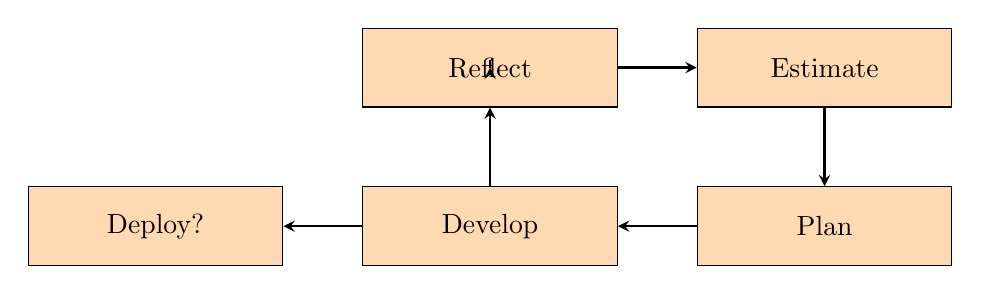
\begin{tikzpicture}[node distance=1cm]
	\node (reqs) [process] {Requirements};
	\node (est) [process, right=of reqs] {Estimate};
	\node (plan) [process, below=of est] {Plan};
	\node (develop) [process, left=of plan] {Develop};
	\node (reflect) [process, above=of develop] {Reflect};
	\node (deploy) [process, left=of develop] {Deploy?};

	\draw [arrow] (reqs) -- (est);
	\draw [arrow] (est) -- (plan);
	\draw [arrow] (plan) -- (develop);
	\draw [arrow] (develop) -- (reflect);
	\draw [arrow] (reflect) -- (reqs);
	\draw [arrow] (develop) -- (deploy);
\end{tikzpicture}\\\\
This diagram shows that the process is iterative and incremental as we loop back to the start (with a reflection stage) at the end of every development cycle (iteration).
\subsection{Iteration Stages}
\subsubsection{Agile Practices: User Stories}
Agile takes a different approach to requirements gathering. Instead of using a typical requirements specification, requirements are gathered as `user stories'.
\begin{center}
	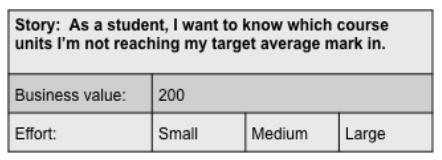
\includegraphics[scale=0.5]{user-story.png}
\end{center}
\subsubsection{Estimation}
You are given a set of user stories. Before starting to build, you need to decide what to commit to.
\subsubsection{Planning}
Next, you select the stories from your backlog that you will implement in the iteration. The key here is balancing business value achieved, effort expended, dependencies between stories and the amount of learning gained from implementation effort. Documenting the plan can be done by using a task board.
\subsubsection{Development and Showcase}
Next you implement as many of your selected stories as you can and show the customer what you've achieved. The customer will sign off the stories that have been completed satisfactorily and the rest will be put into the backlog for the next iteration.
\subsubsection{Feedback}
Finally we hit the feedback stage where we receive feedback from both the customer and the development team in the hope that the feedback will improve out process for the next iteration.

\section{The Trouble with Big Upfront Requirements Gathering}
\subsection{Advantages of a BUFR Specification}
\begin{itemize}
	\item Means that the initial requirements can be put into a contract so that the customer is tied to them.
	\item As the requirements won't change, you can work out how much it'll cost and how much time it'll take to build.
\end{itemize}
These advantages are based on some assumptions:
\begin{itemize}
	\item There exists a reasonably well-defined set of requirements if we only take the time to understand them.
	\item Changes to requirements will be small enough that we can manage them without substantially rethinking or revising our plans.
	\item Software innovation and the research and development that is required to create a significant new software application can be done on a predictable scale.
\end{itemize}
If all of these assumptions hold it should be fine to proceed with big upfront requirements gathering.
\subsection{Change in Software Requirements}
What can cause requirements to change?
\begin{itemize}
	\item The customer can change the budget.
	\item They don't know what they want through the whole process.
	\item The scale of the project may change.
	\item There may be a big technology change.
\end{itemize}
Given these, there is one major source of change that is often unacknowledged. Changes can occur even on projects where the requirements are not very volatile when the change is in our understanding (customer \& developers) of what the requirements are as we build the system.

\subsection{Written Requirements Specifications}
BUFR means that you have to write the specification down. Written specifications are a lot of work and have to constantly be kept up-to-date. Natural language is inherently imprecise and ambiguous which leads to people jumping to their preferred interpretation which can cause problems further down the development process where the developers and the customer had a different understanding of the meaning of the specification. People are also psychologically less likely to question the correctness of something if it is written down.

On an agile project we gather requirements throughout the whole project rather than just at the beginning. We also put off requirements gathering for as long as possible. We try to stray away from writing down all of the requirements in a formal requirements document and we use face-to-face conversations between customers and business analysts/developers to communicate requirements to the people writing the code.

The key points here are that BUFR would be the best way to gather requirements if the underlying assumptions held in practice. Unfortunately they do not. Requirements are rarely clear from the outset, they change frequently, we learn the most about them after delivery and written documents are usually more trouble than they are worth.

Instead, agile approaches aim for just in time/just enough iterative, incremental requirements gathering based on conversations between customers and developers.

\section{How Do We Know What to Build?}
To avoid BUFR, we need an approach to requirements gathering that is:
\begin{itemize}
	\item Just-in-time, just-enough
	\item Iterative AND incremental
	\item Value driven
\end{itemize}
An iterative process model is, at its simplest, one in which an artefact is created by repeating a process more than once. This implies that the artefact created by a single pass through the process is incomplete. In an incremental process, we divide the system to be built into smaller units that are each in themselves complete. In each pass through the process, we work to create one of these units (called increments), so that at the end of each pass we have a version of the system that delivers only a part of the full requirements but which is complete in that it can be executed and maybe even deployed and used.

Our highest priority is to satisfy the customer through early and continuous delivery of valuable software. There are several value oriented agile practices we can use to aid in this such as impact mapping, user stories and road-maps but it all depends on having a good understanding of what value you are aiming for. An aim is like a behaviour change:
\begin{itemize}
	\item Get more visitors to our website
	\item Get more customers to buy our product
	\item Get claim assessors to make fewer mistakes when deciding to pay-out for insurance claims
\end{itemize}
Our first step is to clarify the value. We should ask what impacts are we aiming to achieve and link it to something concrete such as saving money/time. Denne and Cleland-Huang suggest the following types of value for software:
\begin{itemize}
	\item Revenue generation
	\item Cost saving
	\item Competitive differentiation
	\item Brand projection
	\item Enhanced loyalty
\end{itemize}

\subsection{User Stories}
A user story is any brief description of the functionality the software system we are building might usefully have. All of the following are acceptable examples:
\begin{itemize}
	\item I want to see my current average overall mark for the semester and the year
	\item I can find out which course units I'm signed up for
	\item Students are reminded when the deadline for making course choices is approaching
	\item Show list of the course units the student can pick from
\end{itemize}
We want to specify features that are about to be implemented in detail and specify a high level picture for features that will not be implemented for a while. User stories can be written at different levels of abstraction which can cover these ideas. Compare the following user stories:
\begin{itemize}
	\item I want to watch films on demand over the internet.
	\item I want to manage the collection of films I've purchased for on demand viewing.
	\item I want to continue watching a film I've already started to watch, from the point I left off.
\end{itemize}
As you can see, the first user story is at a high level of abstraction whereas the final one is quite a low level story.

Each story should deliver a useful, usable version of the system (an increment).Each story should describe a (thin) \textbf{end-to-end slice} of functionality. Many beginning story writers find it helpful to use a template when writing stories. We will use the Connextra template:
\begin{center}
	As a \textit{type of person}, I want \textit{some functionality} so that \textit{some value is created}
\end{center}
On a real agile project, the use of a story template is optional. We are using it because it is well known, prompts us to include important elements of the story and avoids `blank page syndrome'. Some examples of this template in use are below:
\begin{itemize}
	\item As an existing customer, I want to browse the list of newly acquired films, so that I can quickly discover films I might want to watch.
	\item As a company purchaser, I want to know what the most popular new films are, so that I can focus our licensing discussions on those that will maximise return to the company.
	\item As a media purchases manager, I want to compare projected and actual revenue from each film, so that I can make better decisions about how to adjust our models for the next quarter.
\end{itemize}

\subsubsection{Gathering User Stories}
Some ways of gathering user stories are story writing workshops, impact mapping and story mapping. Story mapping is where we tell the story of how the system will be used and then add details of how the software will support the story.

\subsubsection{The INVEST Properties for Useful User Stories}
As writing good stories can sometimes be difficult, Bill Wake coined this mnemonic for the properties that we want out user stories to have:
\begin{itemize}
	\item \textbf{Independent:} the stories should be able to be implemented in any order (i.e. they shouldn't be technically dependent on each other)
	\item \textbf{Negotiable:} no aspect of the story is deemed unchangeable throughout the lifetime of the project.
	\item \textbf{Valuable:} the story should have real value to some customer/stakeholder.
	\item \textbf{Estimable:} it should be possible to estimate the size of the story.
	\item \textbf{Small/Appropriately Sized:} stories should be sized relative to the iteration size the team is using.
	\item \textbf{Testable:} It should be possible to devise a concrete and unambiguous test that can tell us whether the story has been implemented or not.
\end{itemize}

\section{How Do We Know What to Build Next?}
\end{document}
